%%%%%%%%%%%%%%%%%%%%%%%%%%%%%%%%%%%%%%%%%%%%%%%%%%%%%%%%%%%%%%%%%%%%%%%%%%%%%%
% University of Bristol presentation theme based on the PowerPoint template
%
% Copyright (c) 2012, 2020 David A.W. Barton (david.barton@bristol.ac.uk)
% All rights reserved.
%
% The latest version of this theme can be found at
%   https://github.com/db9052/UoB-beamer-theme
% 
%%%%%%%%%%%%%%%%%%%%%%%%%%%%%%%%%%%%%%%%%%%%%%%%%%%%%%%%%%%%%%%%%%%%%%%%%%%%%%

\documentclass[aspectratio=169]{beamer}
    % Possible aspect ratios are 16:9, 16:10, 14:9, 5:4, 4:3 (default) and 3:2
    % (Remember to remove the colon, i.e., 16:9 becomes the option 169)

\usetheme{UoB}
% If lualatex is used then Rockwell, Latin Modern math, and Arial are used as
% per the UoB style. If pdflatex is used then Concrete, Euler math, and
% Helvetica are used as the closest alternatives. 

%%%%%%%%%%%%%%%%%%%%%%%%%%%%%%%%%%%%%%%%%%%%%%%%%%%%%%%%%%%%%%%%%%%%%%%%%%%%%%
\title[Quantum Scrambling]{Scrambling Encoded Information}
\subtitle{Physics Research Project}
\author{Samuel A. Hopkins}
\institute{Theoretical Physics MSci}
\date{23rd March 2023}



\begin{document}

% Available frame options:
%   leftcolor, rightcolor: set the colour of the left or right panel
%   leftimage, rightimage: put a (cropped) image in the left or right panel
%   div: set the location of the divider between left and right panels
%   urlcolor: set the colour of the url

% Other commands available:
%   \logo{X}: choose the logo to display (logo, white logo, or black logo)
%   \urltext{X}: change the url for each slide

% All standard University of Bristol colours are available:
%   UniversityRed, CoolGrey, BrightAqua, BrightBlue, BrightOrange, BrightPurple,
%   BrightPink, BrightLime, DarkAqua, DarkBlue, DarkOrange, DarkPurple,
%   DarkPink, DarkLime

\begin{frame}[leftcolor=CoolGrey,rightcolor=UniversityRed,div=0.8\paperwidth]
  \titlepage
\end{frame}

%%%%%%%%%%%%%%%%%%%%%%%%%%%%%%%%%%%%%%%%%%%%%%%%%%%%%%%%%%%%%%%%%%%%%%%%%%%%%%
\lecture{Lecture 1}{01}


%%%%%%%%%%%%%%%%%%%%%%%%%%%%%%%%%%%%%%%%%%%%%%%%%%%%%%%%%%%%
\begin{frame}[plain]
  A plain slide that might be useful for displaying large figures
\end{frame}

%%%%%%%%%%%%%%%%%%%%%%%%%%%%%%%%%%%%%%%%%%%%%%%%%%%%%%%%%%%%
\begin{frame}[div=0.675\paperwidth]{Some bullet points (with an image!)}
  % The image can either be in the frame options or as below
  \rightimage{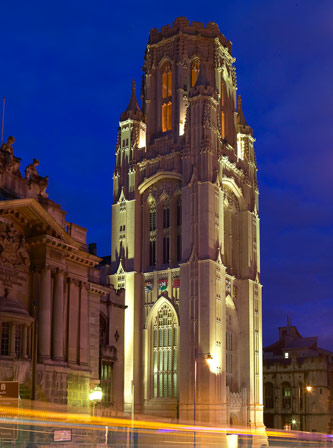
\includegraphics[trim=0 0 20mm 0,clip,height=\paperheight]{WillsMemorialBuilding.jpg}}
  Use a better quality image though...
  \begin{itemize}[<+->]
  \item These will get revealed one by one
    \begin{itemize}
    \item Indented bullets
    \item Some more indented bullets
    \end{itemize}
  \item Another bullet point
  \item Yet another bullet point
  \end{itemize}
\end{frame}

%%%%%%%%%%%%%%%%%%%%%%%%%%%%%%%%%%%%%%%%%%%%%%%%%%%%%%%%%%%%
\begin{frame}[div=0.6\paperwidth]{Another smaller image}
  \rightimage{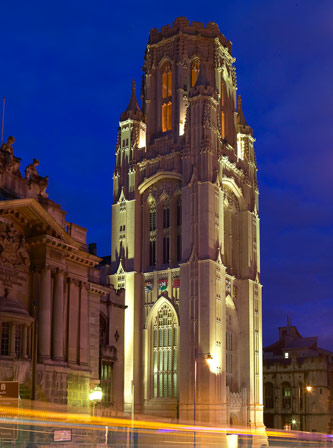
\includegraphics[angle=-90,origin=b,width=0.4\paperwidth]{WillsMemorialBuilding.jpg}}
  \begin{minipage}{0.625\linewidth}
    \raggedright
    Smaller images are centred on the slide and can be used for interesting effects.
    \medskip

    Lorem ipsum dolor sit amet, consectetur adipisicing elit, sed do eiusmod
    tempor incididunt ut labore et dolore magna aliqua. Ut enim ad minim veniam,
    quis nostrud exercitation ullamco laboris nisi ut aliquip ex ea commodo
    consequat. Duis aute irure dolor in reprebhenderit in voluptate velit esse
    cillum dolore eu fugiat nulla pariatur. Excepteur sint occaecat cupidatat non
    proident, sunt in culpa qui officia deserunt mollit anim id est laborum.
  \end{minipage}
\end{frame}




%%%%%%%%%%%%%%%%%%%%%%%%%%%%%%%%%%%%%%%%%%%%%%%%%%%%%%%%%%%%
\end{document}

%%%%%%%%%%%%%%%%%%%%%%%%%%%%%%%%%%%%%%%%%%%%%%%%%%%%%%%%%%%%%%%%%%%%%%%%%%%%%%
